% =====================================================================
%  ViralJEPA -- Deep Learning course project report, University of Padova
%  Compile with pdfLaTeX + BibTeX (Overleaf: default settings are fine).
%  Needs: references.bib, figures/exp02_pretrain_curves.png,
%         figures/exp03_pretrain_curves.png
% =====================================================================
\documentclass[10pt,twocolumn,a4paper]{article}

\usepackage[utf8]{inputenc}
\usepackage[T1]{fontenc}
\usepackage{lmodern}
\usepackage[margin=1.8cm]{geometry}
\usepackage{microtype}
\usepackage{amsmath,amssymb}
\usepackage{graphicx}
\usepackage{booktabs}
\usepackage{tabularx}
\usepackage{caption}
\usepackage{xcolor}
\usepackage[numbers,sort&compress]{natbib}
\usepackage[colorlinks=true,linkcolor=blue!45!black,citecolor=blue!45!black,
            urlcolor=blue!45!black]{hyperref}

\captionsetup{font=small,labelfont=bf}
\setlength{\parskip}{0.2em}
\setlength{\columnsep}{6mm}
\setlength{\bibsep}{0pt plus 0.2ex}        % tighter reference list
\setlength{\textfloatsep}{10pt plus 2pt minus 2pt}
\setlength{\dblfloatsep}{10pt plus 2pt minus 2pt}
\setlength{\dbltextfloatsep}{12pt plus 2pt minus 2pt}
\bibliographystyle{unsrtnat}

% Placeholder for the numbers that the pending run will produce.
\newcommand{\tbd}{\textcolor{gray}{$\cdot$}}

\begin{document}

% Title set across both columns.
\twocolumn[{%
\begin{center}
  {\LARGE\bfseries ViralJEPA: Joint-Embedding Predictive Pretraining\\[3pt]
   for Viral Sequence Detection in Human Metagenomes\par}
  \vspace{8pt}
  {\large Luca Grigolin\par}
  \vspace{3pt}
  {\small Deep Learning, University of Padova\par}
\end{center}
\vspace{10pt}
}]

% =====================================================================
\section{Introduction}
% =====================================================================

Metagenomic sequencing of a clinical sample returns DNA from everything the
specimen contained: the human host, its bacteria, and any viruses present.
Assigning the assembled contigs to an origin is normally done by alignment
against reference databases, but a large fraction of viral sequence matches
nothing known, the problem called viral dark
matter~\cite{krishnamurthy2017darkmatter}. Alignment-free classifiers instead
learn what viral sequence \emph{looks like}: VirFinder~\cite{ren2017virfinder}
works from $k$-mer frequencies, DeepVirFinder~\cite{ren2020deepvirfinder} and
Seeker~\cite{auslander2020seeker} apply neural networks to raw sequence, and
VirSorter2~\cite{guo2021virsorter2} and geNomad~\cite{camargo2024genomad}
combine learned signals with protein markers.

\paragraph{ViraMiner and ViraMiner-CB.}
\citet{tampuu2019viraminer} framed the task on human clinical metagenomes: 19
sequencing experiments over sample types such as serum, skin and condylomata,
with contigs cut into 300\,bp pieces and labelled by BLAST, about 2\% of them
viral, split 80/10/10. Their network runs two branches over the one-hot
sequence, a \emph{pattern} branch (convolution, global max pooling) asking
whether a motif is present and a \emph{frequency} branch (convolution, global
average pooling) asking how often motifs occur, trained separately and merged.
It reaches a test AUROC of 0.923 against 0.875 for a random forest on 6-mer
counts, with 90\% precision at 32\% recall. A second experiment removes every
anellovirus from training and tests on 1{,}348 anellovirus contigs among
26{,}296 non-viral ones, where the frequency branch reaches 0.755; since
anelloviruses are diverse, ubiquitous commensals of the human
virome~\cite{kaczorowska2020anello}, this held-out family is a meaningful probe
of generalisation to an unseen taxon. A later project of this
course~\cite{pivotto2024viraminercb} kept the same data and layout and replaced
the first convolutional layer of a new branch with an Inception-style
block~\cite{szegedy2015inception}, a 1D and a 2D convolution in parallel on the
one-hot input; its best configuration reached 0.922, comparable to ViraMiner but
not above it, which its authors attributed mainly to the absence of branch
pretraining. Both datasets and splits are reused unchanged here.

\paragraph{What this project adds.}
Both models are supervised convolutional networks trained on about 2\%
positives, and both plateau near 0.92 AUROC. Two observations drive this work.
Convolutions see only a local window, whereas a
Transformer~\cite{vaswani2017attention} on top of convolutional motif tokens can
relate motifs anywhere in the contig. And labelled viral contigs are scarce
while unlabeled genomes are abundant, which is exactly the asymmetry
self-supervised pretraining
exploits~\cite{ji2021dnabert,zhou2024dnabert2,dallatorre2025nt,nguyen2023hyenadna}.
The report presents a CNN--Transformer baseline (Section~\ref{sec:vm3}), the
case for a joint-embedding predictive objective (Section~\ref{sec:why}), a
leakage-controlled corpus (Section~\ref{sec:corpus}), the pretraining method and
the failed runs that shaped it (Section~\ref{sec:method}), and the evaluation
protocol (Section~\ref{sec:eval}). All code is
public~\cite{grigolin2026viraminer3,grigolin2026corpus,grigolin2026viraljepa}.

% =====================================================================
\section{ViraMiner3: a CNN--Transformer baseline}\label{sec:vm3}
% =====================================================================

\paragraph{Architecture and training.}
A one-hot sequence of shape $300\times4$ enters a multi-kernel stem: four Conv1D
layers in parallel with kernels of 5, 7, 11 and 15\,bp, 72 filters each, stride
2, GELU~\cite{hendrycks2016gelu}, concatenated into 150 tokens of 288 features
and normalised with BatchNorm~\cite{ioffe2015batchnorm}. The kernels span short
motifs up to about five codons, so the stem plays the role of ViraMiner's two
branches at several scales at once. A learned CLS token and learned positions are
added and a 6-layer pre-norm~\cite{xiong2020prenorm} Transformer (8 heads, width
288) mixes the tokens; the CLS output passes a LayerNorm~\cite{ba2016layernorm}
and an MLP ($288\to512\to128\to1$), for 6.3\,M parameters. Because positives are
rare the loss is focal~\cite{lin2017focal} ($\alpha=0.75$, $\gamma=2$, smoothing
0.05). AdamW~\cite{loshchilov2019adamw} uses $10^{-4}$ for the stem and head and
$5\cdot10^{-5}$ for the Transformer, which is frozen for 5 epochs so the random
head cannot push large gradients into the attention layers; the schedule is a
5-epoch warm-up then cosine decay~\cite{loshchilov2017sgdr}, at most 120 epochs,
patience 15 on validation AUROC, batch 128, fp16~\cite{micikevicius2018mixed}.
Augmentation is a reverse complement at probability 0.5 and a shift of up to
$\pm5$\,bp, since strand and cut points carry no label information. The operating
threshold maximises F1 on validation.

\paragraph{Choosing the baseline.}
A controlled trial compared this architecture with four variants changing either
the motif encoder or the token aggregation (Table~\ref{tab:vm3}). Shrinking the
stem to two kernels costs a point of AUROC, so the range of kernel sizes matters
more than filters per kernel; enlarging it to 512-dimensional tokens triples the
parameters and performs \emph{worse}, its collapse in precision (0.48) showing
the larger model overfitting a 2\%-positive training set. Local attention and
attention pooling leave test AUROC unchanged while lowering validation AUROC.
Neither component is the bottleneck, so the baseline was kept: at 0.932 it
improves on ViraMiner (0.923) and ViraMiner-CB (0.922) on the same split.

\begin{table*}[t]
\centering
\caption{ViraMiner3 architecture trial on the ViraMiner \texttt{fullset} test
split (551 viral contigs out of 26{,}405). Checkpoints are selected by validation
AUROC; precision, recall and F1 refer to the viral class at the best-F1
validation threshold. Single seed.}
\label{tab:vm3}
\footnotesize
\begin{tabular}{lrcccccc}
\toprule
Variant & Params & Val AUROC & Test AUROC & Test AP & Prec. & Rec. & F1 \\
\midrule
\textbf{Baseline: 4 kernels $\times$ 72, CLS} & 6.27\,M & \textbf{0.931} & \textbf{0.932} & 0.563 & 0.672 & \textbf{0.465} & \textbf{0.549} \\
Local attention, $\pm64$ tokens            & 6.27\,M & 0.926 & 0.930 & \textbf{0.566} & 0.683 & 0.437 & 0.533 \\
CLS $+$ attention pooling                  & 6.41\,M & 0.926 & 0.932 & 0.560 & \textbf{0.695} & 0.434 & 0.534 \\
2 kernels (7, 11) $\times$ 144             & 6.26\,M & 0.921 & 0.927 & 0.528 & 0.636 & 0.416 & 0.503 \\
4 kernels $\times$ 128, token width 512    & 19.34\,M & 0.920 & 0.925 & 0.517 & 0.484 & 0.454 & 0.468 \\
\midrule
ViraMiner~\cite{tampuu2019viraminer}       & --- & --- & 0.923 & --- & 0.90 & 0.32 & --- \\
ViraMiner-CB~\cite{pivotto2024viraminercb} & --- & --- & 0.922 & --- & 0.84 & 0.32 & --- \\
\bottomrule
\end{tabular}
\end{table*}

% =====================================================================
\section{Why a joint-embedding predictive objective}\label{sec:why}
% =====================================================================

Genomic foundation models are pretrained almost exclusively by reconstructing
their input. DNABERT~\cite{ji2021dnabert}, DNABERT-2~\cite{zhou2024dnabert2} and
the Nucleotide Transformer~\cite{dallatorre2025nt} predict masked tokens in the
style of BERT~\cite{devlin2019bert}; HyenaDNA~\cite{nguyen2023hyenadna} and
Evo~\cite{nguyen2024evo} predict the next nucleotide. At single-base resolution much of genomic DNA is locally close to
incompressible, so a reconstruction loss spends most of its capacity on
base-level detail. The signal separating viral from host sequence is of a
different kind: organism-level regularities such as oligonucleotide composition,
which Karlin and Burge called a genomic signature~\cite{karlin1995signature},
codon usage and motif statistics. These are exactly what ViraMiner's frequency
branch and the $k$-mer baselines exploit, and what a per-base objective is least
pressed to encode.

Joint-Embedding Predictive Architectures~\cite{lecun2022path} predict the
\emph{representation} of a hidden part of the input instead of its raw content,
letting the model discard detail it cannot predict.
I-JEPA~\cite{assran2023ijepa} predicts the latent features of masked image blocks
from a visible context block, with targets from an exponential-moving-average
(EMA) copy of the encoder, and learns semantic features without hand-crafted
augmentations; V-JEPA~\cite{bardes2024vjepa} and
V-JEPA\,2~\cite{assran2025vjepa2} carry the recipe to video, where pixel-level
prediction is hopeless. data2vec~\cite{baevski2022data2vec} showed the principle
holds across speech, vision and language when the target is a contextualised
representation averaged over the top layers of an EMA teacher rather than a
single layer. JEPA-DNA~\cite{larey2026jepadna} brought it to genomics, adding a
latent objective on a global embedding predicted from a span-masked context on
top of the native generative loss, with consistent linear-probing and zero-shot
gains across 17 tasks and three backbones; its stated motivation is that
reconstruction ``can prioritize low-level details over more abstract semantic
structure''.

These sit inside the wider family of joint-embedding
approaches~\cite{balestriero2023cookbook}: BYOL~\cite{grill2020byol} and
SimSiam~\cite{chen2021simsiam} predict one view's embedding from another's with
an asymmetric predictor and a stop-gradient and no negatives;
DINO~\cite{caron2021dino} and iBOT~\cite{zhou2022ibot} self-distil a global token
alongside masked patch tokens; VICReg~\cite{bardes2022vicreg} replaces negatives
with explicit variance and covariance terms. All share one failure mode: an
encoder can satisfy a latent-matching loss by emitting constant or low-rank
outputs, studied as dimensional
collapse~\cite{jing2022dimensional,tian2021understanding}. For DNA,
DNABERT-S~\cite{zhou2024dnaberts} showed that treating two fragments of one
genome as a positive pair yields embeddings clustering by species, close to what
is needed here, since separating viral from human or bacterial sequence is a
coarse species-level distinction. Section~\ref{sec:lessons} shows that
transferring such an objective naively is nonetheless not enough.

% =====================================================================
\section{The pretraining corpus}\label{sec:corpus}
% =====================================================================

What the unlabeled data contains is a design decision as consequential as the
objective. The corpus built for this project~\cite{grigolin2026corpus},
\texttt{corpus\_v3}, holds 4{,}000{,}000 windows of 300\,bp, matching the
downstream input length exactly so that no change of resolution occurs between
pretraining and fine-tuning. Three requirements shaped it: span the sequence
domains a human metagenome actually contains, on both sides of the decision;
contain no evaluation sequence, or a frozen probe would measure memorisation; and
leave one viral family completely unseen, preserving the anellovirus benchmark as
a genuine test of generalisation to a new taxon.

\subsection{Sources}

Five public reference collections were used (Table~\ref{tab:sources}), each
chosen to fill a specific gap. \emph{RefSeq viral}~\cite{oleary2016refseq} gives
broad taxonomic coverage of curated viral genomes; records whose description
mentions a phage are routed to the prokaryotic-virus category and the rest to the
eukaryotic one. \emph{NCBI Virus}~\cite{hatcher2017ncbivirus} adds depth where RefSeq is thin: complete genomes annotated with a human host, restricted to fourteen
families occurring in clinical metagenomes plus the human retroviruses. Public
archives are heavily skewed towards a few intensively sequenced species, so at
most ten genomes are kept per ICTV species; without this cap a handful of
pathogens would dominate the category. \emph{UHGV}~\cite{camargo2025uhgv}, the
unified human gut virome catalogue, contributes the phages that dominate real gut
samples and that RefSeq represents poorly~\cite{shkoporov2019phages}, restricted
to representatives rated \emph{Complete} or \emph{High-quality} by
CheckV~\cite{nayfach2021checkv} so that fragmentary assemblies do not enter as if
they were genomes.

The negatives come from two sources. \emph{UHGG}~\cite{almeida2021uhgg} supplies
1{,}000 gut species representatives at completeness $\ge90\%$ and contamination
$\le5\%$, selected round-robin across phyla so Firmicutes and Bacteroidota do not
crowd out the rest. \emph{T2T-CHM13v2.0}~\cite{nurk2022t2t} supplies human
sequence; the complete assembly was preferred because it resolves centromeres and
satellite arrays absent from GRCh38 that appear readily in real data and that a
classifier must learn not to flag. Finally 180{,}000 windows come from
\texttt{fullset\_train} with labels discarded, carrying the sequencing artefacts
and error profile of the target domain that no reference genome reproduces.

\begin{table*}[t]
\centering
\caption{Sources of \texttt{corpus\_v3}. Records and Mbp are counted after
filtering. The two virus categories draw on RefSeq and on NCBI Virus or UHGV
jointly, so their window counts are reported in Table~\ref{tab:mix} rather than
per source.}
\label{tab:sources}
\footnotesize
\begin{tabularx}{\textwidth}{llXr}
\toprule
Source & Category & Records kept & Records / Mbp \\
\midrule
RefSeq viral & virus, euk.\ and prok. & all, minus 175 anellovirus records and 139 duplicated in NCBI Virus & 19{,}275 / 580 \\
NCBI Virus & virus, eukaryotic & complete genomes, human host, $\le10$ per ICTV species; Anelloviridae dropped & 1{,}266 / 33 \\
UHGV & virus, prokaryotic & vOTU representatives of CheckV quality Complete or High-quality; 927 Anelloviridae dropped & 57{,}734 / 2{,}598 \\
UHGG v2.0.2 & bacteria & 1{,}000 species representatives, $\ge90\%$ complete, $\le5\%$ contaminated, balanced over phyla & 92{,}449 contigs / 2{,}612 \\
T2T-CHM13v2.0 & human & all 25 sequences of the analysis set & 25 / 3{,}117 \\
ViraMiner train & ViraMiner & random rows of \texttt{fullset\_train}, labels removed & --- \\
\bottomrule
\end{tabularx}
\end{table*}

\subsection{Window extraction and composition}

Each category receives a fixed share of the four million windows
(Table~\ref{tab:mix}). Viruses take just over half the corpus although they are a
small minority of any real sample: the encoder should model viral sequence well,
and the class prior belongs to the fine-tuned classifier, not to the pretraining
distribution. Within a category, windows are allocated to genomes in proportion
to length, capped at 50\,kb for every non-human source. Without the cap, jumbo
phages and poxviruses, two or three orders of magnitude longer than a
circovirus, would absorb most of the budget.

Windows are drawn at uniformly random positions. A window containing any
character outside ACGT is redrawn, up to four attempts, so that masking and
one-hot encoding stay well defined; soft-masked repeats are upper-cased and
retained, because repetitive human sequence is exactly what the model must learn
not to flag. Every window is reverse-complemented with probability 0.5, since a
contig may be sequenced from either strand. Each window keeps an identifier
\texttt{category|source|record|start|strand}. The \texttt{record} field, naming
the genome, contig or chromosome the window came from, is what makes the
paired-view objective of Section~\ref{sec:cls} possible: it is the only grouping
information the model ever receives, and the category is never exposed to it.

\begin{table*}[t]
\centering
\begin{minipage}[t]{0.45\textwidth}
\centering
\caption{Composition of \texttt{corpus\_v3}.}
\label{tab:mix}
\small
\begin{tabular}{lrr}
\toprule
Category & Share & Windows \\
\midrule
Viruses, prokaryotic & 32.5\% & 1{,}300{,}000 \\
Human                & 25.0\% & 1{,}000{,}000 \\
Bacteria, gut        & 20.0\% &   800{,}000 \\
Viruses, eukaryotic  & 18.0\% &   720{,}000 \\
ViraMiner, unlabeled &  4.5\% &   180{,}000 \\
\midrule
Total                & 100\%  & 4{,}000{,}000 \\
\bottomrule
\end{tabular}
\end{minipage}\hfill
\begin{minipage}[t]{0.52\textwidth}
\centering
\caption{Leakage screens. A window is discarded when at least 10\% of its
canonical $k$-mers occur in the screen set.}
\label{tab:screen}
\small
\begin{tabular}{p{2.2cm}p{2.5cm}cr}
\toprule
Applied to & Screen set & $k$ & Removed \\
\midrule
External genomes & \texttt{fullset} val.\ and test, anell.\ test & 31 & 95{,}340 \\
ViraMiner windows & anellovirus test split & 31 & 25{,}829 \\
All windows & anellovirus test positives & 15 & 447 \\
\bottomrule
\end{tabular}
\end{minipage}
\end{table*}

\subsection{Leakage control}

Any window reproducing an evaluation contig would let a probe or a fine-tuned
model score well for the wrong reason. Windows are therefore screened against
sets of canonical $k$-mers and discarded when at least 10\% of their $k$-mers
appear in the screen set (Table~\ref{tab:screen}). At $k=31$ this fires on
near-exact overlap while chance matches are effectively impossible. Most removals
are human windows (93{,}397), as expected since the non-viral part of ViraMiner
is largely human; because the anellovirus test split re-partitions the same pool
as \texttt{fullset\_train}, the ViraMiner-derived windows were screened against
it separately, removing a further 25{,}829.

Anelloviruses are excluded three times over: by taxonomic annotation, by a
regular expression over record descriptions, and by a screen at $k=15$ against
the anellovirus test positives. The shorter word is deliberate, since 15-mers
survive roughly 10\% divergence often enough to exceed the threshold while chance
matches stay at 1--2\% of a window, which catches relatives of the test family
that taxonomy alone would miss. The draw runs at 1.3 times the target count to
absorb these rejections, and the survivors are trimmed and shuffled.

Three limitations remain. RefSeq contains plant and insect viruses that never
occur in human samples; the per-species cap is taxonomic rather than
sequence-based, so near-identical strains can still repeat; and every bacterial
genome comes from the gut, while ViraMiner also draws on skin and cervical
samples, so the bacterial negatives are narrower than those met at test time.

% =====================================================================
\section{ViralJEPA}\label{sec:method}
% =====================================================================

\subsection{What the earlier runs taught}\label{sec:lessons}

Three experiments preceded the current design. \emph{exp01} applied a token-level
JEPA on the ViraMiner training set alone and fine-tuned to a test AUROC of 0.915,
below the supervised baseline: too little data, and no reason for the
representation to generalise beyond it. \emph{exp02} and \emph{exp03} pretrained
on the corpus of Section~\ref{sec:corpus} following JEPA-DNA, monitored
throughout with a frozen linear probe, a logistic regression fitted on
mean-pooled features of the ViraMiner training split. That probe has an unusually
strong reference point: a \emph{randomly initialised} encoder already reaches an
AUROC near 0.83, because mean-pooled random convolutions act like random
projections of $k$-mer composition, and composition is most of the signal. Any
pretraining that fails to clear this bar has destroyed information.

\begin{figure*}[t]
\centering
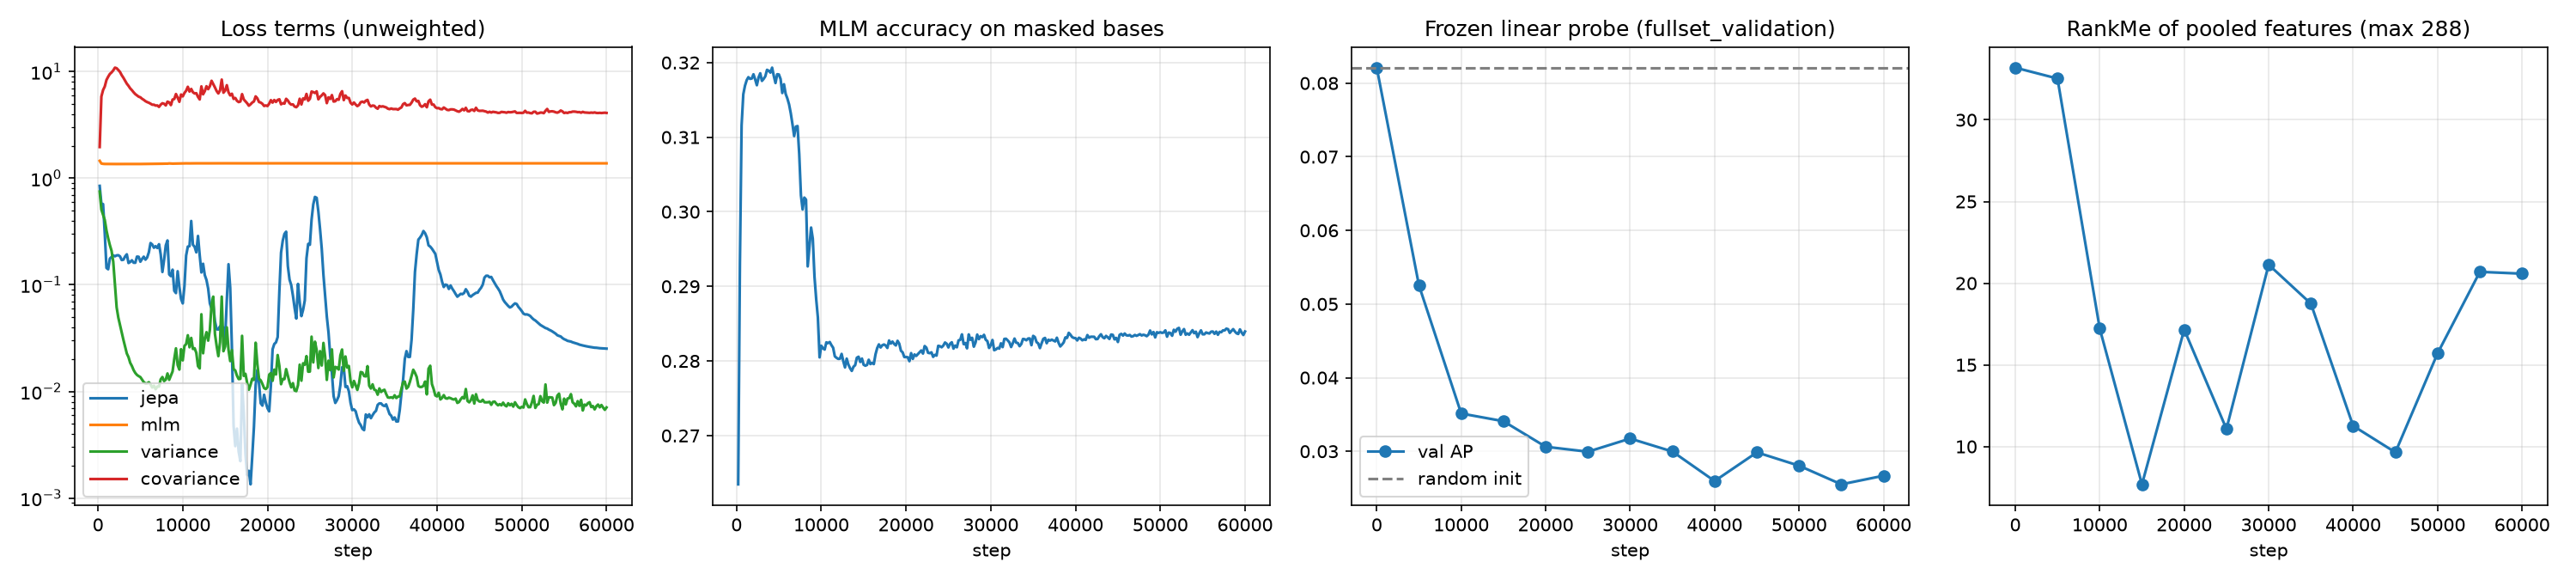
\includegraphics[width=0.80\textwidth]{figures/exp02_pretrain_curves.png}\\[3pt]
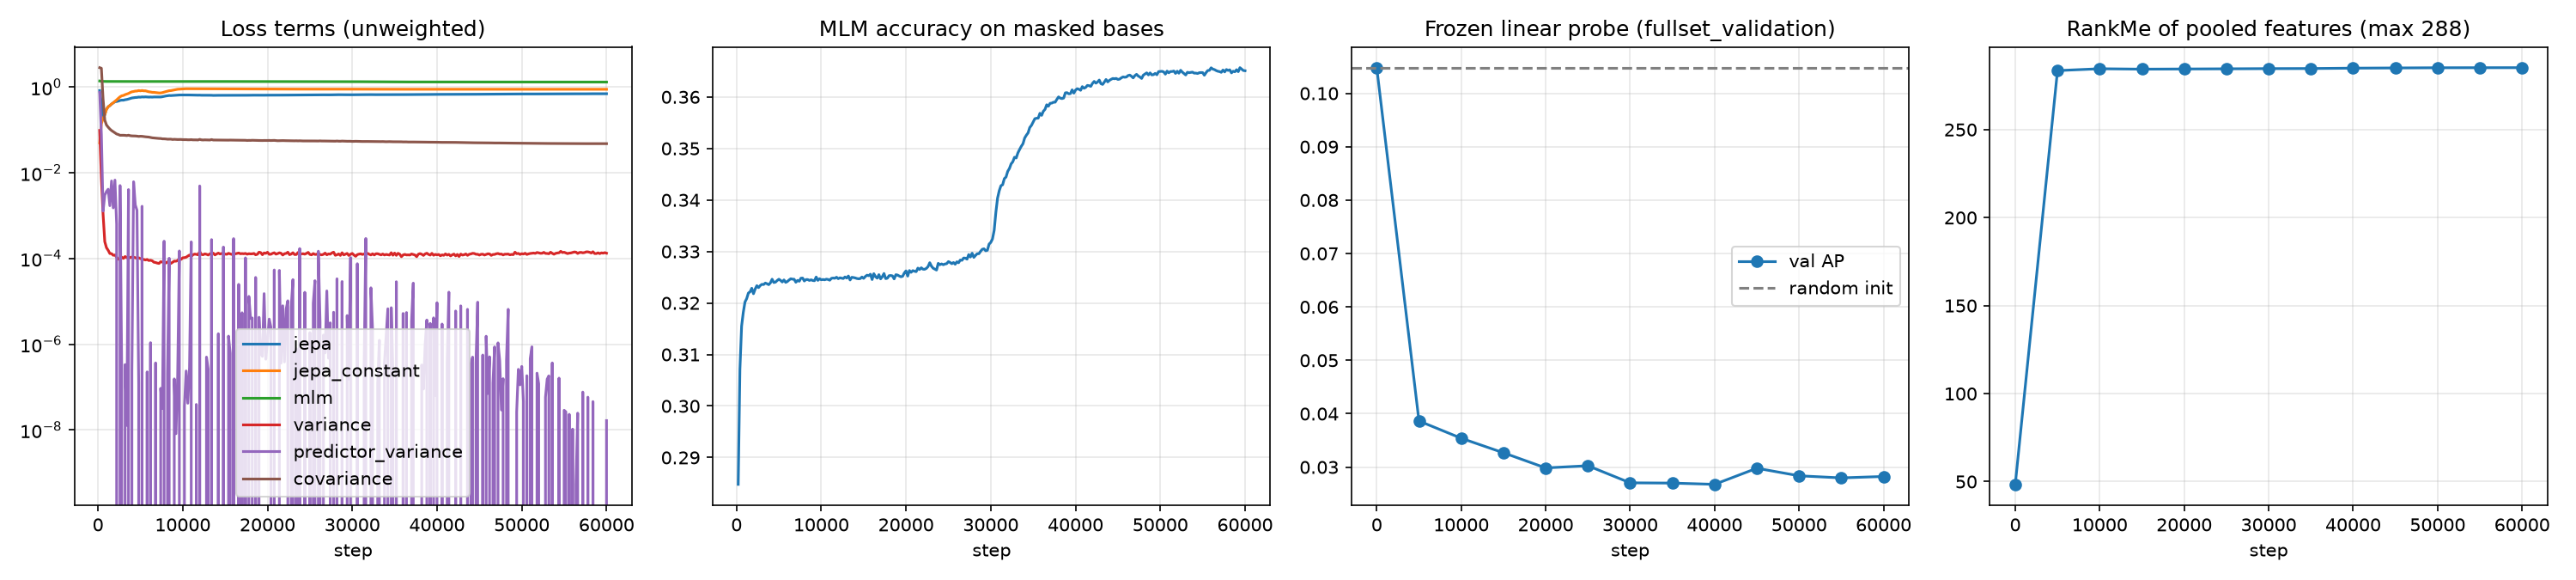
\includegraphics[width=0.80\textwidth]{figures/exp03_pretrain_curves.png}
\caption{Pretraining diagnostics for exp02 (top) and exp03 (bottom): unweighted
loss terms, MLM accuracy on masked bases, frozen linear-probe average precision
on \texttt{fullset\_validation} with the random-initialisation level as a dashed
line, and RankMe~\cite{garrido2023rankme} of the pooled features (maximum 288).
The two runs fail in opposite directions. In exp02 the effective rank falls from
33 to about 20, a dimensional collapse. In exp03 it saturates at 285 of 288, a
near-isotropic code. In both the probe ends far below the random encoder.}
\label{fig:collapse}
\end{figure*}

In \emph{exp02} (Figure~\ref{fig:collapse}, top) the VICReg terms were applied to
the predictor's output only. The predictor ends in a LayerNorm, which rescales
whatever it receives, so the penalties were satisfied however degenerate the
encoder beneath had become, and the encoder underwent dimensional
collapse~\cite{jing2022dimensional}: RankMe fell from 33 to 21 and probe AUROC
from 0.80 to 0.56. Fine-tuning from it cost five points of AUROC against random
initialisation (0.875 versus 0.924).

\emph{exp03} (Figure~\ref{fig:collapse}, bottom) moved the variance hinge onto
the encoder's own mean-pooled output, pooled the JEPA target over the masked
spans only as in I-JEPA, and replaced the stem's BatchNorm with a LayerNorm,
since batch statistics differ between masked and clean inputs and are not carried
across by the EMA update. It failed in the opposite direction, instructively. The
pooled vector is a mean of 150 tokens that each leave a LayerNorm, and such a
mean can only have large variance across the batch if the tokens of a sequence
all point the same way. The model duly made them do so: the cosine between a
token and its sequence mean rose to 0.97. The covariance penalty then spread
those per-sequence vectors into a near-isotropic, input-sensitive code, RankMe at
285 of 288, with the targets of different sequences nearly orthogonal. The JEPA
loss \emph{rose} over training, from 0.19 to 0.70, and the probe fell to 0.62.
Fine-tuning recovered the supervised level (0.920 against 0.919) but gained
nothing: the pretrained weights were simply overwritten.

Two conclusions carry into the present design. Anti-collapse terms must not act
on the representation that will later be classified, because satisfying them is
not the same as making that representation useful. And the context and target
encoders must not see the same window, since nothing in that arrangement rewards
invariance to anything meaningful.

\subsection{Encoder and masking}

The encoder is the ViraMiner3 architecture of Section~\ref{sec:vm3} with a
LayerNorm stem and the CLS token kept \emph{inside} the Transformer, exactly
where the classifier will read it. Two kinds of token are hidden from the context
encoder; each token covers 2\,bp.

\textbf{JEPA spans} are contiguous and non-overlapping, on a schedule growing
linearly from one or two spans covering 10--20\% of the tokens to one to four
covering 20--30\%. Span masking follows SpanBERT~\cite{joshi2020spanbert}, the
block masking of I-JEPA~\cite{assran2023ijepa} and the scheduler of
JEPA-DNA~\cite{larey2026jepadna}, whose ratios reach 50\%; they were lowered
because on a 150-token window a 50\% span hides 150 consecutive bases, half the
contig, leaving a context too thin to predict from.

\textbf{Scattered MLM tokens} are single tokens outside the spans, each hidden
with probability 0.15 as in BERT~\cite{devlin2019bert}, so their neighbours stay
visible and their bases remain predictable from local context. This corrects
exp02, where the MLM loss was scored inside the long spans and never improved on
base frequencies: the middle of a 150\,bp gap carries no recoverable local
information for a single-nucleotide model trained from scratch.

About 28\% of tokens are hidden at the start of training and 36\% at the end.
Hidden bases are set to N \emph{before} the stem, so no visible token's
overlapping kernel can see them, and the tokens are replaced by a learnable mask
embedding \emph{after} it, as in BERT and MAE~\cite{he2022mae}. The CLS token is
never masked.

\subsection{Token objective: latent prediction of the hidden spans}

The target encoder is an EMA copy of the context encoder,
$\bar\theta\leftarrow m\,\bar\theta+(1-m)\,\theta$, with $m$ rising linearly from
0.996 to 1 as in BYOL and I-JEPA; it sees the unmasked window $A$. Following
data2vec~\cite{baevski2022data2vec}, the target $y_i$ for token $i$ is the
average of the outputs of the last $K=3$ Transformer blocks, each passed through
a LayerNorm without affine parameters, which gives a richer and more stable
target than the final layer alone. A narrow predictor $g_\phi$ (four pre-norm
layers at half the encoder width, three heads, fixed sinusoidal positions, as in
JEPA-DNA) receives the context CLS and tokens with mask embeddings at the hidden
positions and predicts each masked span token individually, as in I-JEPA:
\begin{equation}
\mathcal{L}_{\text{jepa}}
 =\frac{1}{|S|}\sum_{i\in S}\frac{1}{d}
   \bigl\lVert\, g_\phi\bigl(\mathrm{ctx}(A)\bigr)_i-\operatorname{sg}(y_i)\,\bigr\rVert_2^2 ,
\end{equation}
with $S$ the set of span tokens and $\operatorname{sg}$ the stop-gradient. Giving
every position its own target is what keeps the tokens apart: predicting 150
distinct vectors is impossible for an encoder whose tokens have collapsed onto
one, which is exactly the solution exp03 found. A linear MLM head on the context
tokens predicts the two bases under each scattered token by cross-entropy,
$\mathcal{L}_{\text{mlm}}$, keeping the tokens accurate at base level in the same
spirit as JEPA-DNA retaining the native generative loss.

\subsection{CLS objective: learning what windows of a genome share}\label{sec:cls}

The sequence-level objective is attached to the CLS token rather than to a pooled
summary of the tokens. This is the central change from exp03, and it mirrors the
division of labour in DINO and iBOT~\cite{caron2021dino,zhou2022ibot}, where a
global token carries the image-level objective while patch tokens carry the local
one. The CLS receives three signals.

\paragraph{A second view from the same genome.}
For each window $A$ a second window $B$ is drawn from the same record, and both
are augmented independently. $A$ and $B$ share no bases and may lie on opposite
strands, so whatever they have in common is a property of the organism they came
from: composition, codon usage, GC skew. This is the positive-pair definition of
DNABERT-S~\cite{zhou2024dnaberts}, and it plays the role random crops play in
SimCLR~\cite{chen2020simclr} and DINO. Only record membership is used; the
category is never shown. Single-window records, the ViraMiner rows, fall back to
a re-augmented copy of $A$.

\paragraph{Self-distillation across the two views.}
Following BYOL~\cite{grill2020byol}, the CLS of the masked $A$ passes through a
projector $h$ (an MLP to 1024 dimensions, with LayerNorm where BYOL uses
BatchNorm, which would drift between the online and EMA copies) and a predictor
$q$, and must match the EMA target's projection of the clean $B$:
\begin{equation}
\mathcal{L}_{\text{global}}
 = 1-\cos\!\bigl(q(h(c_A)),\ \operatorname{sg}\bigl(\bar h(\bar c_B)\bigr)\bigr).
\end{equation}
The asymmetric predictor together with the slowly moving target is what keeps
BYOL-style methods from collapsing without negative
pairs~\cite{tian2021understanding,chen2021simsiam}. Reading the \emph{masked}
$A$ adds a further demand: the CLS must identify the source organism from roughly
70\% of an already short window.

\paragraph{VICReg on the projector, not on the representation.}
A variance hinge, requiring each dimension to have standard deviation at least
$\gamma=1$ across the batch, and a covariance penalty on the squared off-diagonal
entries, act on $z_A=h(c_A)$~\cite{bardes2022vicreg}. Unlike exp02, which
regularised the predictor, and exp03, which regularised the pooled representation
itself, these terms now act on the expander output, which is where VICReg
prescribes them. The projector absorbs the pressure to be spread out and
decorrelated, and the CLS beneath it is free to keep whatever structure is
actually useful.

\paragraph{A composition target.}
A linear head on the CLS of $A$ predicts the 4-mer frequency profile of $B$,
counted over both strands, under a KL divergence. Computed directly from the DNA,
this target cannot drift or collapse and is informative from the first step,
unlike the EMA target, which is near-random early on. Predicting $B$'s profile
rather than $A$'s stops the head solving the task by counting visible bases: a
single 300\,bp window gives a noisy estimate, so the best available prediction is
the organism's average profile, the same quantity the self-distillation term asks
for. Regressing a hand-crafted descriptor follows
MaskFeat~\cite{wei2022maskfeat}, which regresses HOG features, and aims the
objective squarely at the genomic signature~\cite{karlin1995signature} the
frequency branch and $k$-mer baselines rely on.

The total objective is the weighted sum
\begin{equation}
\mathcal{L}=\mathcal{L}_{\text{jepa}}+\mathcal{L}_{\text{global}}
           +\mathcal{L}_{\text{kmer}}+\mathcal{L}_{\text{mlm}}
           +\lambda_{v}\,\mathcal{L}_{\text{var}}+\lambda_{c}\,\mathcal{L}_{\text{cov}},
\end{equation}
with $\lambda_v=1$ and $\lambda_c=0.04$. Pretraining runs 60{,}000 steps at batch
size 512, roughly 7.7 passes over the corpus, with AdamW at a peak learning rate
of $5\cdot10^{-4}$ cosine-decayed after 3{,}000 warm-up steps, weight decay 0.05
excluding biases, normalisation parameters, positional embeddings and the mask
and CLS tokens, gradient clipping at 1, and bf16 precision. Each loss is logged beside the value it would
take if the model predicted the batch mean for every sequence, so a term counts
as carrying information only when it falls clearly below that baseline, a
diagnostic added after exp02's JEPA loss of 0.025 proved to mean nothing.

% =====================================================================
\section{Evaluation protocol}\label{sec:eval}
% =====================================================================

The pretrained encoder is judged in two ways: a frozen linear probe, which asks
what the representation contains without adaptation, and full fine-tuning, which
asks whether pretraining helps the end task. Both compare against a randomly
initialised encoder of identical architecture under an identical recipe. That
control is essential here, since a random encoder is already a competitive
$k$-mer feature extractor.

\paragraph{Frozen linear probe.}
A logistic regression is fitted on standardised features of
\texttt{fullset\_train} and scored on \texttt{fullset\_test}, features taken from
clean windows and averaged over both strands. Two read-outs are reported: the CLS
output, which the classifier uses, and the mean of the token outputs, which exp02
and exp03 measured. Alongside AUROC and average precision,
RankMe~\cite{garrido2023rankme} gives the effective rank of the feature matrix,
the statistic that exposed both collapse modes in Figure~\ref{fig:collapse}. The
probe also runs every 5{,}000 pretraining steps, so a run destroying information
can be stopped early (Table~\ref{tab:probe}).

\begin{table}[t]
\centering
\caption{Frozen linear probe: fitted on \texttt{fullset\_train}, scored on
\texttt{fullset\_test}, reverse-complement averaged features. Results pending.}
\label{tab:probe}
\footnotesize
\setlength{\tabcolsep}{4pt}
\begin{tabular}{llccc}
\toprule
Encoder & Read-out & AUROC & AP & RankMe \\
\midrule
Random init. & CLS       & \tbd & \tbd & \tbd \\
Random init. & mean-pool & \tbd & \tbd & \tbd \\
ViralJEPA    & CLS       & \tbd & \tbd & \tbd \\
ViralJEPA    & mean-pool & \tbd & \tbd & \tbd \\
\bottomrule
\end{tabular}
\end{table}

\paragraph{Fine-tuning tasks.}
Two tasks are run. \texttt{fullset} trains on \texttt{fullset\_train}, selects on
\texttt{fullset\_validation} and reports on \texttt{fullset\_test} (551 viral of
26{,}405): the in-distribution setting. \texttt{anell} trains on the anellovirus
training split, with any window identical to a test window removed and a 10\%
stratified validation split held out, and reports on the anellovirus test split
(1{,}348 viral of 27{,}644). It needs its own fine-tune because its test
positives also occur in \texttt{fullset\_train}, and it is the more informative
of the two: anelloviruses are absent from the corpus, the fine-tuning data and
the screens alike, so it measures transfer to a family never seen.

\paragraph{Fine-tuning recipe.}
The classifier is the encoder plus the MLP head of Section~\ref{sec:vm3} reading
the CLS output, trained exactly as the supervised baseline and with the
Transformer frozen for the first 5 epochs. With a pretrained encoder that freeze
gives the standard linear-probe-then-fine-tune order, which preserves pretrained
features that full fine-tuning from the first step tends to
distort~\cite{kumar2022lpft}. Checkpoints are selected on validation average
precision rather than AUROC, since with 2\% positives AP is the more
discriminating. Each task--initialisation pair runs with three seeds, every
metric is reported plain and with reverse-complement test-time averaging, worth
one to two points in the earlier runs, and bootstrap 95\% confidence intervals
accompany test AUROC and AP (Table~\ref{tab:finetune}).

\begin{table*}[t]
\centering
\caption{Fine-tuning results, mean $\pm$ standard deviation over three seeds.
RC-TTA denotes reverse-complement test-time averaging; precision, recall and F1
refer to the viral class at the best-F1 validation threshold. Results pending;
the ViraMiner3 row is the supervised reference from Table~\ref{tab:vm3}.}
\label{tab:finetune}
\footnotesize
\begin{tabular}{llcccccccc}
\toprule
Task & Init. & Seeds & AUROC & AP & AUROC RC & AP RC & F1 RC & Prec. RC & Rec. RC \\
\midrule
\texttt{fullset} & ViraMiner3 & 1 & 0.932 & 0.563 & --- & --- & 0.549 & 0.672 & 0.465 \\
\texttt{fullset} & random     & 3 & \tbd & \tbd & \tbd & \tbd & \tbd & \tbd & \tbd \\
\texttt{fullset} & ViralJEPA  & 3 & \tbd & \tbd & \tbd & \tbd & \tbd & \tbd & \tbd \\
\midrule
\texttt{anell}   & random     & 3 & \tbd & \tbd & \tbd & \tbd & \tbd & \tbd & \tbd \\
\texttt{anell}   & ViralJEPA  & 3 & \tbd & \tbd & \tbd & \tbd & \tbd & \tbd & \tbd \\
\bottomrule
\end{tabular}
\end{table*}

\paragraph{Ablations.}
Three switches isolate the design's contributions, each a separate pretraining
run followed by the same two fine-tunes. Replacing the same-genome second view
with a re-augmented copy of the same window tests whether paired windows, rather
than ordinary augmentation, are what the CLS objective needs. Setting the 4-mer
weight to zero tests how much comes from the explicit composition target rather
than from self-distillation. Using only the final Transformer block as the token
target tests the data2vec-style multi-layer target.

% =====================================================================
\section{Conclusions}
% =====================================================================

This project set out to test whether self-supervised pretraining can push viral
sequence detection beyond supervised training on the ViraMiner data. Three
results hold independently of the pending run.

First, architecture gives a modest but real improvement. Replacing the two pooled
convolutional branches with convolutional motif tokens followed by a Transformer
raises test AUROC from 0.923 to 0.932, and a controlled trial showed that neither
a larger motif encoder nor a different aggregation adds more. The remaining gap
is not a capacity problem.

Second, much of the real work lies in the corpus. Assembling four million windows
is easy; making them a sound basis for evaluation is not. Capping genomes by
length and species stops a handful of over-sequenced organisms from defining what
the model takes a virus to be, and the $k$-mer screens are what keep the
anellovirus benchmark meaningful.

Third, and most instructive, the two failed runs were not failures of the JEPA
idea but of where its constraints were applied. exp02 regularised the predictor
and let the encoder collapse to rank 21; exp03 regularised the pooled
representation and produced the mirror image, a near-isotropic code of rank 285
built from tokens collapsed onto one vector per sequence. Both satisfied their
objectives completely while destroying the composition signal a random encoder
supplies for free. The lesson generalises: an anti-collapse term applied to the
representation that will later be classified constrains the wrong object, and a
loss value means nothing until compared against what predicting the batch mean
would score.

The present design follows from that diagnosis: the sequence-level objective is
carried by a CLS token, regularised through a projector rather than directly and
supervised by a second window of the same genome, so the invariance learned is
organism identity rather than an arbitrary code, while the token-level objective
predicts each hidden position separately against a multi-layer target, which
structurally prevents tokens from collapsing together. Whether this finally beats
a randomly initialised encoder is the open question, and the anellovirus task is
where the answer matters most: an in-distribution gain could come from
optimisation alone, but a gain on an unseen viral family would mean the encoder
has learned something about viral sequence as such. If no gain appears there
either, the honest conclusion will be that at this model and corpus scale the
composition signal a random convolutional stem already provides is close to what
300\,bp of DNA can offer, and that progress must come from longer contigs or
substantially larger pretraining rather than from a better objective.

{\scriptsize
\bibliographystyle{unsrtnat}
\bibliography{references}
}

\end{document}
